\documentclass{article}

\usepackage{graphicx}
\usepackage{hyperref}
\usepackage{bm}

%----------------------------------------------------------------------------------------
%	ASSIGNMENT INFORMATION
%----------------------------------------------------------------------------------------

\title{CS5200: Homework \#1} % Title of the assignment

\author{Matthew Whitesides\\ \texttt{mbwxd4@mst.edu}} % Author name and email address

\date{\today} % University, school and/or department name(s) and a date

%----------------------------------------------------------------------------------------

\begin{document}

\maketitle % Print the title
 
\begin{enumerate}
  \item Signed statement on last page. 
  
  \item Question 2.
  \begin{enumerate}
    \item The age of the Earth is estimated at least 4.3 and commonly estimated at \textbf{4.54 billion years} old.

    \item The age of the Solar System is estimated between \textbf{4.53 and 4.58 billion years} old.

    \item The age of the Milky Way Galaxy is estimated at \textbf{11 to 13 billion years} old.

    \item The age of the universe is estimated at \textbf{10 to 15 billion years} old.
    \begin{itemize}
      \bibitem{usgs} 
      (Questions A - D): Dalrymple, G. Brent.
      \textit{The Age of the Earth}.
      \textit{\href{https://pubs.usgs.gov/gip/geotime/age.html}{https://pubs.usgs.gov/gip/geotime/age.html}}
      Stanford University Press, 492p, 1991.
    \end{itemize}

    \item The fate of the earth will probably be ended by our sun expanding into the earth in about 7 billion years putting the earth's lifespan at around \textbf{11 billion years} old.
    \begin{itemize}
      \bibitem{Ward} 
      Ward, Peter.
      \textit{The life and death of planet Earth}.      
      Holt, First edition, page 158, January 1, 2004.
    \end{itemize}

    \item There are many ways earth could become uninhabitable by humans however ignoring man-made disasters, and unplanned events such as an asteroid, the earth will naturally go through temperature cycles that would destroy civilization. A man killing ice age is hard to predict but could begin anywhere from \textbf{one to tens of thousands of years} from now, or millions, the last one was only 11 thousand years ago. Recent human activities have increased the climate decay and instability, and to preserve the climate as long as possible we would need to reduce our carbon emissions, and possibly on the survival of the species perspective would eventually need to figure out ways to massively heat or cool the earth survive natural global temperature cycles.
    \begin{itemize}
      \bibitem{Revkin} 
      Revkin, Andrew C.
      \textit{When Will the Next Ice Age Begin?}.
      \textit{\href{https://www.nytimes.com/2003/11/11/science/when-will-the-next-ice-age-begin.html}{https://www.nytimes.com/2003/11/11/science/when-will-the-next-ice-age-begin.html}}
      New York Times, Nov. 10, 2003, Section F, Page 6.
    \end{itemize}
    \begin{itemize}
      \bibitem{William} 
      Reville, William.
      \textit{How long will the human species survive on Earth?}.
      \textit{\href{https://www.irishtimes.com/news/science/how-long-will-the-human-species-survive-on-earth-1.2885564}{https://www.irishtimes.com/news/science/how-long-will-the-human-species-survive-on-earth-1.2885564}}
      Thu, Dec 8, 2016.
    \end{itemize}

    \item The estimated lifespan of the solar system will be about \textbf{11 billion years}. In around five billion years from now, the sun will enter a red giant phase and slowly expand outward for another billion years before exhausting all its energy.
    \begin{itemize}
      \bibitem{Redd} 
      Redd, Nola Taylor.
      \textit{Red Giant Stars: Facts, Definition and the Future of the Sun}.
      Schröder, Connon Smith, R. (2008).
    \end{itemize}

    \item There are many theories about how the universe will end but a commonly used one is related to heat death. In anywhere from \textbf{1 to 100 trillion years}, there will not be enough matter/energy for stars to form and the universe will contain mainly black holes which themselves will disappear eventually.
    \begin{itemize}
      \bibitem{Yun} 
      Wang, Yun.
      \textit{RCurrent observational constraints on cosmic doomsday}.
      Journal of Cosmology and Astro-Particle Physics. 2004 (12)
    \end{itemize}

    \item If there are 31536000 seconds in a year then (($2^{64}$ - 1) / 31536000) is equal to about \textbf{585 billion years} wich if we go with the lower estimate of the universe lifespan is around \textbf{59\%}.
  \end{enumerate}

  \item Question 3. 
  \begin{enumerate}
    \item Assuming the letters can be used more than once we'd have $26^{9}$ combinations or \textbf{5.43 trillion}.
    \item Using the same logic we'd have \bm{$K^{9}$} \textbf{combinations}.
    \item So if $K^{9} = 9000000000$ then $K = \sqrt[9]{9000000000}$, so $K = 12.765$ or you'd need a \textbf{13 character} alphabet to work.
    \item \bm{$K\times (K - 1)^{n - 1}$}. Pretty much it's the same except the first character is K possible letters and every other character is K - 1 possibilities.
    \item Assuming we're going with small but not trying to min/max the use of paper too much, if we use 10px font, standard 8.5 x 11 letter size (not double sided), at 300px/inch printing, with a small margin of 2px between lines we'll get $(11\times 300) / 12 = 275$ words per page. So \textbf{9 billion / 275 = 32.7 million pages}.
    \item Looking at Amazon I see I can get Amazon Basics paper 5,000 sheets for \$44.99. So $(32700000 / 5000) * 44.99 = 294234.6$ so it'd be a cool \textbf{\$294,234.60} assuming Amazon will sell us 6,540 boxes of paper. Now the best selling file cabinet I see on Amazon is a 3 drawer, 18 inch deep cabinet. Amazon lists the same paper in a 500 sheet reem as being 2 inches thick so we could get $(250\times 18)\times 3 = 13500$ per cabinet. So we'd need $32700000 / 13500 = 2422.22$ or \textbf{2,423} cabinets.
    \item They planned on about \textbf{15 thousand} years to finish the project. However they didn't say how many people would be working on it for that estimate so we can only assume it'd take one person that long. If they hope to finish the project in one persons lifespan given they start at 18 years old and retire at 60 years old (42 years per person) and assuming they accounted for the person working probably wouldn't work 24/7 in that original estimate, they'd need \bm{$15000 / 42 = 357.14$} people (maybe a part time person for the 0.14).
    \item The computer people estimated \textbf{one thousand} days (or 86400000 seconds) to finish, and saying there's 9 billion combinations (which isn't exact but they didn't give all details about their alphabet in the story) it'd have to do \bm{$86400000 / 9000000000 = 0.0096$} \textbf{words/sec} which seems fast but maybe they print inline and on a large sheet with laser printers. 
    \item Good story, I like the twilight zone kinda ending. Although seems odd they'd be that afraid of Monks at the end. Does make you think about how little you use large numbers in everday life and how futile it'd be to try to do an entire large task without breaking it down into small peices. Really anything over a 100 or so becomes nonsense in most peoples mind I feel.
  \end{enumerate}

\end{enumerate}

\pagebreak

\begin{figure}
  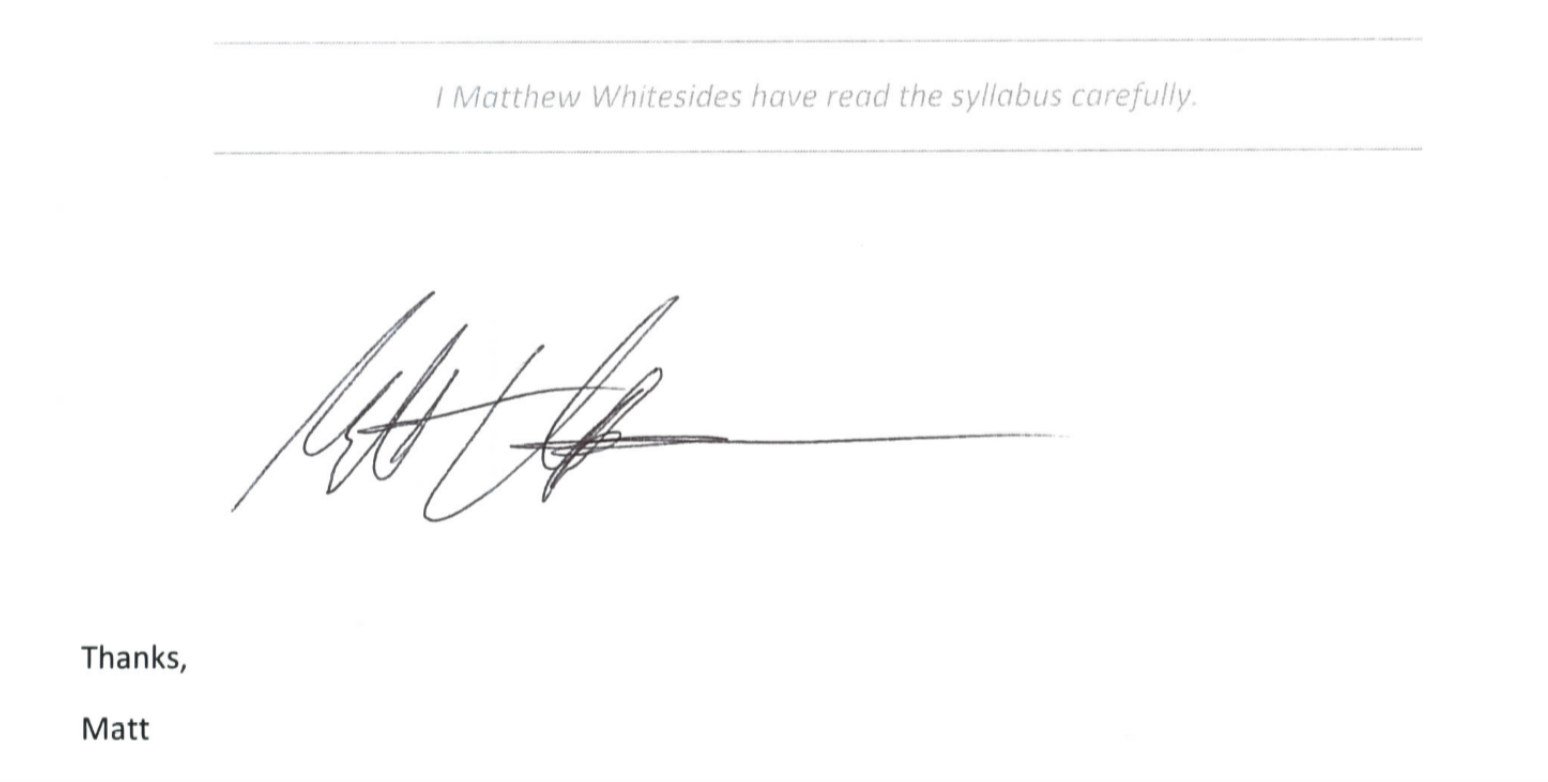
\includegraphics[width=\linewidth]{Statement.png}
  \label{fig:Statement}
\end{figure}

\end{document}
